\documentclass{report}
\usepackage{graphicx} % Required for inserting images
\usepackage{amsmath} % For mathematical equations
\usepackage{python} % For including Python code
\usepackage{xcolor} % For setting colors
\usepackage{listings} % For including code snippets
\usepackage{amssymb} % For mathematical symbols
\usepackage{pgfplots} % For plotting graphs 
\usepackage{tikz} % For drawing diagrams
\usepackage{float} % Add this line at the beginning of the document

\lstset{ %
  language=Python,             % Choose the language of the code
  basicstyle=\ttfamily,        % Code font style
  keywordstyle=\color{blue},   % Keywords color
  commentstyle=\color{gray},   % Comments color
  stringstyle=\color{red},     % Strings color
  numbers=left,                % Line numbers on the left
  numberstyle=\tiny\color{gray},  % Style of line numbers
  frame=single,                % Adds a frame around the code
  breaklines=true,             % Line break for long code lines
  captionpos=b                 % Position of caption (below the code)
}

\pgfplotsset{compat=1.16} % Set the version of pgfplots

\title{Interdisciplinary Mathematics and Computer Science \\
\large A Pedagogical Approach to Teaching Both Fields }
\author{Derek Neilson}
\date{\today}


\begin{document}

\tableofcontents

\maketitle

\chapter{Preface}
\section{Preface}\label{sec:preface}

\subsection{Abbreviations}

The following abbreviations are used throughout this paper:

\subsubsection{Computer Science Abbreviations}

\begin{tabular}{ll}
    \textbf{CS} \& Computer Science \\
    \textbf{DS} \& Data Structures \\
    \textbf{OOP} \& Object-Oriented Programming \\
    \textbf{AI} \& Artificial Intelligence \\
    \textbf{DBMS} \& Database Management System \\
    \textbf{ML} \& Machine Learning \\
    \textbf{OS} \& Operating System \\
    \textbf{API} \& Application Programming Interface \\
\end{tabular}

\subsubsection{Mathematics Abbreviations}

\begin{tabular}{ll}
    \textbf{DM} \& Discrete Mathematics \\
    \textbf{P \& C} \& Probability and Combinatorics \\
    \textbf{S \& L} \& Sets and Logic \\
    \textbf{T \& F} \& Truth and Falsity \\
    \textbf{FFT} \& Fast Fourier Transform \\
    \textbf{LCM} \& Least Common Multiple \\
    \textbf{GCD} \& Greatest Common Divisor \\
    \textbf{PDF} \& Probability Density Function \\
\end{tabular}

\subsubsection{General Abbreviations}

\begin{tabular}{ll}
    \textbf{STEM} \& Science, Technology, Engineering, and Mathematics \\
    \textbf{UI} \& User Interface \\
    \textbf{UX} \& User Experience \\
    \textbf{BFS} \& Breadth-First Search \\
    \textbf{DFS} \& Depth-First Search \\
    \textbf{RSA} \& Rivest-Shamir-Adleman (encryption algorithm) \\
\end{tabular}

\subsection{Figures} \listoffigures % Correct LaTeX command to print the list of figures

\subsection{Tables} \listoftables

\subsection{Code} \lstlistoflistings

\subsection{Introduction}

This paper is a collection of thoughts and ideas that have been developed over the past few years. The concepts presented here are the result of my experiences as a computer science student. Although I have always been interested in mathematics, it wasn't until I approached the subject from a computer science perspective that I fully appreciated its beauty. This paper is an effort to share some of the insights I have gained through this interdisciplinary lens.

\subsection{Acknowledgements}

This work was completed independently, but I am deeply grateful to Weber State University for providing the resources and opportunities that have enabled me to pursue my interests. I would also like to thank my family and friends for their support and encouragement. Finally, I extend my gratitude to the authors of the textbooks and papers I have referenced throughout this work. Their contributions have been invaluable in helping me develop my own ideas.

\subsection{Abstract}

This paper explores the relationship between mathematics and computer science, focusing on the ways in which that students can benefit from an interdisciplinary approach to these fields. The paper begins by comparing elementary mathematical concepts to their computer science counterparts and beginner programming concepts to their mathematical equivalents. It then discusses the benefits of teaching mathematics and computer science together, including the development of problem-solving skills, the promotion of creativity, and the enhancement of students' understanding of both subjects. As the paper progresses, it delves into more advanced topics, such as the connections between discrete mathematics and computer science, the role of algorithms in both fields, and the ways in which computer science can be used to solve complex mathematical problems. The paper concludes by emphasizing the importance of interdisciplinary education and encouraging educators to incorporate elements of both mathematics and computer science into their curricula. The goal of this paper is to inspire students and educators alike to explore the connections between these two disciplines and to appreciate the beauty and power of mathematics and computer science when studied together.



    
\chapter{Introduction}

\section{Introduction}

Computer Science (\textbf{CS}) and mathematics are two closely related disciplines that share concepts and techniques. Both fields focus on the study of abstract structures and the development of algorithms for manipulating these structures. Despite their close relationship, the two disciplines have traditionally been taught separately, with minimal emphasis on the connections between them. This paper explores the deep interrelationship between \textbf{CS} and mathematics, highlighting the ways in which students can benefit from a more integrated, interdisciplinary approach to these fields.

The paper begins by comparing elementary mathematical concepts to their \textbf{CS} counterparts and beginner programming concepts to their mathematical equivalents. This comparison serves to illustrate the similarities and differences between the two disciplines and to lay the groundwork for a more in-depth exploration of their connections. Python code snippets are included throughout the paper to provide concrete examples of the concepts being discussed. These code snippets are intended to be accessible to readers with little to no programming experience. Each code snippet is accompanied by a brief explanation of the code and its relevance to the topic at hand. The Math examples are thoroughly explained and are intended to be accessible to readers with little to no mathematical experience. As the paper progresses, it delves into more advanced topics. Some topics covered may be challenging for readers without a strong background in mathematics or \textbf{CS}, but the paper is designed to be accessible to a wide audience.
    


\chapter{Mathematical and Programming Fundamentals}\label{ch:mathematical-foundations}

\section{Introduction}

In this section, we will explore the fundamental concepts of mathematics and programming that serve as the building blocks for more advanced topics in both fields. We will cover topics such as place value, variables, arithmetic operators, and the order of operations. These concepts are essential for understanding the deep connections between mathematics and computer science and will provide a solid foundation for the rest of the paper.

\section{Place Value}

\subsection{Place Value and Number Systems}

A number system is a way of representing numbers. The most common number system is the decimal system, which is also known as the base-10 system. The base-10 system uses ten digits: 0, 1, 2, 3, 4, 5, 6, 7, 8, and 9. The value of a digit in a number depends on its position in the number. For example, in the number 123, the digit 3 is in the ones place, the digit 2 is in the tens place, and the digit 1 is in the hundreds place. The value of the number is calculated by multiplying each digit by its place value and adding the results together. In this case, the value of the number 123 is $1 \times 100 + 2 \times 10 + 3 \times 1 = 100 + 20 + 3 = 123$.

\begin{align*}
    123 &= 1 \times 10^2 + 2 \times 10^1 + 3 \times 10^0 \\
        &= 1 \times 100 + 2 \times 10 + 3 \times 1 \\
        &= 100 + 20 + 3 = 123
\end{align*}

\section{Variables}

\subsection{What is a Variable?}
A variable is a named storage location in a computer's memory that holds a value. The value of a variable can change during the execution of a program. Variables are used to store data that is used by the program, such as numbers, strings, and objects. In Python, variables are created by assigning a value to a name using the assignment operator, which is the equals sign (=). For example, the following code creates a variable named x and assigns it the value 10:

\begin{lstlisting}
    # Create a variable named x and assign it the value 10
    x = 10
\end{lstlisting}
    
In this code, the variable \lstinline|x| is created and assigned the value \lstinline|10|. You will notice that there is some text following a hash symbol (\lstinline|# |) this is a comment in Python. Comments are used to explain the code and are ignored by the Python interpreter. Comments are useful for documenting code and making it easier to understand.

\subsection{Mathematical Variables}
In mathematics, variables are used to represent unknown values or values that can change. Variables are typically denoted by letters, such as $x$, $y$, and $z$. For example, in the equation $y = 2x + 3$, $x$ and $y$ are variables. The value of $y$ depends on the value of $x$. If $x$ is 1, then $y$ is 5. If $x$ is 2, then $y$ is 7. In this way, variables in mathematics are similar to variables in programming. They both represent values that can change.

\subsection{Commonalities and Differences}
Variables in mathematics and programming share some commonalities. They both represent values that can change, and they are both used to store data. However, there are some key differences between variables in mathematics and programming. In mathematics, variables are used to represent unknown values or values that can change, while in programming, variables are used to store data that is used by the program. Additionally, variables in programming have a specific type, such as integer, float, or string, while variables in mathematics are more abstract and can represent any type of value.

\section{Arithmetic-operators}

\subsection{Addition (+) and Subtraction (-)}
Addition and subtraction are fundamental arithmetic operations used in both mathematics and programming. 

\subsubsection{Addition}
In mathematics, addition is represented by the plus sign (+), and it combines two numbers to produce a sum. For example, $2 + 3 = 5$. Similarly, in programming, addition is also represented by the plus sign. In Python, this would be written as \lstinline|2 + 3 = 5|. Here's a simple code snippet that demonstrates addition in Python:

\begin{lstlisting}
# Addition
x = 2
y = 3
print(x + y)  # Output: 5
\end{lstlisting}

In this code, the variables \lstinline|x| and \lstinline|y| are assigned the values \lstinline|2| and \lstinline|3|, respectively. The sum of \lstinline|x| and \lstinline|y| is then computed and printed to the console. The \lstinline|print| function outputs the result of the expression \lstinline|x + y|, which is \lstinline|5|.

\subsubsection{Subtraction}

Subtraction, on the other hand, is represented by the minus sign (-) and is used to find the difference between two numbers. In mathematics, for example, $5 - 3 = 2$. In Python, subtraction is represented in the same way, as shown below:

\begin{lstlisting}
# Subtraction
x = 5
y = 3
print(x - y)  # Output: 2
\end{lstlisting}

In this code, the variables \lstinline|x| and \lstinline|y| are assigned the values \lstinline|5| and \lstinline|3|, respectively. The difference between \lstinline|x| and \lstinline|y| is calculated and printed as \lstinline|2|.

In both cases, whether it's addition or subtraction, the operations in Python mirror those in traditional mathematics, making it easy for programmers to apply their knowledge of arithmetic directly in code.

\subsection{Multiplication (*) and Division (/)}

\subsubsection{Multiplication}
Multiplication is another fundamental arithmetic operation that is used in both mathematics and programming. In mathematics, multiplication is represented by the asterisk (*) symbol, and it is used to find the product of two numbers. For example, $2 \times 3 = 6$. Similarly, in programming, multiplication is also represented by the asterisk symbol. Here's an example of multiplication in Python:

\begin{lstlisting}
# Multiplication
x = 2
y = 3
print(x * y)  # Output: 6
\end{lstlisting}

In this code, the variables \lstinline|x| and \lstinline|y| are assigned the values \lstinline|2| and \lstinline|3|, respectively. The product of \lstinline|x| and \lstinline|y| is then computed and printed to the console. The \lstinline|print| function outputs the result of the expression \lstinline|x * y|, which is \lstinline|6|.
\subsubsection{Division}

Division is represented by the forward slash (/) symbol and is used to find the quotient of two numbers. In mathematics, for example, $6 / 3 = 2$. In Python, division is more nuanced due to the different types of division that can be performed. Here's an example of classic division in Python:

\begin{lstlisting}
# Division
x = 5
y = 2
print(x / y)  # Output: 2.5
\end{lstlisting}

In this code, it is important to note that the division operation \lstinline|x / y| results in a floating-point number, such as \lstinline|2.5|, rather than an integer. A floating-point number includes a decimal point, and Python automatically performs floating-point division when the result is not an integer.

In mathematics, dividing two integers may result in a fraction or a decimal, and Python mirrors this behavior by default. For example, dividing \lstinline|5 / 2| in Python will yield \lstinline|2.5|.

This behavior is different in some other programming languages, such as C or Java, where dividing two integers can result in an integer due to integer division. For instance, in C or Java, the operation \lstinline|5 / 2| would result in \lstinline|2|, effectively discarding the fractional part. This difference is important to keep in mind, as it can lead to unexpected results if you're accustomed to integer division in these languages.

\subsection{The Modulo Operator (\%) and Floor Division (//)}

\subsubsection{Modulo Operator (\%)}
The modulo operator (\%) is another arithmetic operator that is used in both mathematics and programming. In mathematics, the modulo operator is used to find the remainder of the division of two numbers. For example, $5 \% 2 = 1$, because when 5 is divided by 2, the remainder is 1. In Python, the modulo operator is also represented by the percent sign (\%). Here's an example of the modulo operator in Python:

\begin{lstlisting}
# Modulo
x = 5
y = 2
print(x % y)  # Output: 1
\end{lstlisting}

In math this is written as $5 \mod 2 = 1$. The modulo operator is particularly useful in programming for tasks such as determining whether a number is even or odd, or for iterating over a sequence of numbers.

\subsubsection{Floor Division (//)}
Floor division (//) is another division operator in Python that is used to find the quotient of two numbers, rounded down to the nearest integer. For example, $5 // 2 = 2$, because the result of dividing 5 by 2 is 2.5, which is then rounded down to 2. Here's an example of floor division in Python:

\begin{lstlisting}
    # Floor Division
    x = 5
    y = 2
    print(x // y)  # Output: 2
\end{lstlisting}
    
Floor division is useful when you want to divide two numbers and obtain an integer result, rather than a floating-point number. In Python, the operator \lstinline|//| performs floor division. The mathematical equivalent of floor division is dividing two numbers and rounding down to the nearest integer, represented as:
    \[
    \lfloor x \div y \rfloor
    \]
For example, the result of \lstinline|5 // 2| is \lstinline|2|, which corresponds to rounding down the result of \lstinline|5 / 2| (which is \lstinline|2.5|) to the nearest integer.

\subsection{Ceiling Division}
Ceiling division is the opposite of floor division. It rounds up to the nearest integer instead of rounding down. In Python, there is no built-in operator for ceiling division, but you can achieve the same result using the math module. Here's an example of ceiling division in Python:

\begin{lstlisting}
# Ceiling Division
import math
x = 5
y = 2
print(math.ceil(x / y))  # Output: 3
\end{lstlisting}

In this code, the math module is imported to access the \lstinline|ceil| function, which rounds a number up to the nearest integer. Notice that there is a dot operator (\lstinline|.|) used to access the \lstinline|ceil| function from the math module. The result of \lstinline|math.ceil(x / y)| is \lstinline|3|, which corresponds to rounding up the result of \lstinline|5 / 2| (which is \lstinline|2.5|) to the nearest integer. We will discuss modules and functions in more detail in later sections for now just know that the math module is a built-in module in Python that provides mathematical functions and constants. The \lstinline|.| operator is used to access functions and constants within a module.

Mathematically, ceiling division is represented as:
\[
\lceil x \div y \rceil
\]

\section{Order of Operations}

\subsection{What is the Order of Operations?}
The order of operations, also known as precedence rules, is a set of rules that determines the order in which mathematical expressions should be evaluated. The order of operations ensures that expressions are evaluated in a consistent and unambiguous manner. The order of operations is as follows:

\begin{enumerate}
    \item Parentheses
    \item Exponents
    \item Multiplication and Division
    \item Addition and Subtraction
    \item Left to Right
\end{enumerate}

\subsection{CS and Math Notation}

\subsubsection{Parentheses}
In both computer science and mathematics, parentheses are used to group expressions and indicate the order in which operations should be performed. Expressions inside parentheses are evaluated first. For example, in the expression $2 \times (3 + 4)$, the addition inside the parentheses is evaluated first, resulting in $2 \times 7 = 14$.

\subsubsection{Exponents}
Exponents are used to raise a number to a power. In mathematics, exponents are denoted by the caret symbol (\^{}) or by superscript notation. For example, $2^3$ represents $2$ raised to the power of $3$, which is $2 \times 2 \times 2 = 8$. In Python, the double asterisk (\lstinline|**|) operator is used for exponentiation. For example, \lstinline|2 ** 3| represents $2$ raised to the power of $3$, which is \lstinline|8|.
\subsubsection{Multiplication and Division}
Multiplication and division have the same precedence level and are evaluated from left to right. For example, in the expression $2 + 3 \times 4$, the multiplication is performed first, resulting in $2 + 12 = 14$. In Python, the multiplication operator (\lstinline|*|) and the division operator (\lstinline|/|) have the same precedence level and are evaluated from left to right.
\subsubsection{Addition and Subtraction}
Addition and subtraction also have the same precedence level and are evaluated from left to right. For example, in the expression $2 + 3 - 4$, the addition is performed first, resulting in $5 - 4 = 1$. In Python, the addition operator (\lstinline|+|) and the subtraction operator (\lstinline|-|) have the same precedence level and are evaluated from left to right.
\subsubsection{Left to Right}
If two operators have the same precedence level, they are evaluated from left to right. For example, in the expression $2 + 3 - 4$, the addition is performed first because addition and subtraction have the same precedence level, and the expression is evaluated from left to right.

\subsection{Conclusion of \\ Mathematical and Programming \\ Fundamentals}
In this section, we have explored the fundamental concepts of mathematics and programming, including place value, variables, arithmetic operators, and the order of operations. We now have a solid foundation in these concepts, which will serve as the building blocks for more advanced topics further in the paper. The examples and explanations provided in this section are intended to familiarize readers with the format and syntax of the paper, as well as to introduce key concepts that will be referenced throughout the paper. The next section will delve into more advanced topics, building on the knowledge gained here to explore the deep connections between mathematics and computer science.



\chapter{Computer Science Foundations}

\section{Introduction}

Computer science is the study of algorithms and data structures. Algorithms are step-by-step procedures for solving problems. Data structures are ways of organizing data so that it can be used efficiently. In this chapter, we will discuss some fundamental concepts in computer science, and how they relate to mathematics.

\section{Algorithms}

An algorithm is a step-by-step procedure for solving a problem. Algorithms can be written in many ways, but they all have the same basic structure. An algorithm consists of a sequence of steps, each of which is executed in turn. The steps may involve performing calculations, making decisions, or repeating a sequence of steps. The goal of an algorithm is to solve a specific problem, such as finding the shortest path between two points, or sorting a list of numbers.

Let's look at an example of an algorithm. The following algorithm adds 10 to a number:

\begin{lstlisting}
def add_ten(number):
    return number + 10

print(add_ten(5))  # Output: 15
\end{lstlisting}

This algorithm takes a number as input, adds 10 to it, and returns the result. We have not covered the syntax of Python yet so let's do so now.

\subsection{Syntax}

Python is a high-level programming language that is widely used in computer science. It is known for its simplicity and readability. That being said, it is important to understand the syntax of Python in order to write algorithms. Here are some basic concepts in Python:

\begin{itemize}
    \item \textbf{Variables}: Variables are used to store data. In Python, variables are created by assigning a value to a name. For example, \texttt{x = 5} creates a variable \texttt{x} and assigns it the value 5.
    \item \textbf{Functions}: Functions are blocks of code that perform a specific task. In Python, functions are defined using the \texttt{def} keyword. For example, \texttt{def add\_ten(number):} defines a function called \texttt{add\_ten} that takes a number as input.
        \begin{itemize}
            \item Functions can also return values. In Python, the \texttt{return} keyword is used to return a value from a function. For example, \texttt{return number + 10} returns the sum of the number and 10.
            \item Functions can also take multiple arguments. For example, \texttt{def add(x, y):} defines a function that takes two arguments.
        \end{itemize}
    \item \textbf{Indentation}: Python uses indentation to define blocks of code. Blocks of code are defined by the level of indentation. For example, the code inside a function definition is indented by four spaces.
    \item \textbf{Comments}: Comments are used to explain code. In Python, comments start with the \texttt{\#} symbol. For example, \texttt{\# This is a comment} is a comment.
    \item \textbf{Output}: The \texttt{print} function is used to output data. For example, \texttt{print(5)} outputs the number 5.
    \item \textbf{Input}: The \texttt{input} function is used to get input from the user. For example, \texttt{x = input("Enter a number: ")} gets a number from the user and stores it in the variable \texttt{x}.
    \item \textbf{Loops}: Loops are used to repeat a block of code. In Python, there are two types of loops: \texttt{for} loops and \texttt{while} loops. For example, \texttt{for i in range(5):} repeats a block of code five times.
    \item \textbf{Conditional statements}: Conditional statements are used to make decisions in code. In Python, conditional statements are defined using the \texttt{if}, \texttt{elif}, and \texttt{else} keywords. For example, \texttt{if x > 5:} makes a decision based on the value of \texttt{x}.
    \item \textbf{Lists}: Lists are used to store multiple items in a single variable. In Python, lists are created using square brackets. For example, \texttt{numbers = [1, 2, 3, 4, 5]} creates a list of numbers.
    \item \textbf{Dictionaries}: Dictionaries are used to store key-value pairs. In Python, dictionaries are created using curly braces. For example, \texttt{person = \{"name": "Alice", "age": 30\}} creates a dictionary of a person.
    \item \textbf{Sets}: Sets are used to store unique items. In Python, sets are created using curly braces. For example, \texttt{numbers = \{1, 2, 3, 4, 5\}} creates a set of numbers.
\end{itemize}

As we go through this chapter, we will expand on these concepts and show how they are used in algorithms. Let's start by looking at some basic algorithms.

\section{Basic Algorithms}

\subsubsection{Pythagorean Theorem}

The Pythagorean theorem states that in a right-angled triangle, the square of the length of the hypotenuse is equal to the sum of the squares of the lengths of the other two sides. In mathematical terms, if $a$ and $b$ are the lengths of the two sides of the triangle that form the right angle, and $c$ is the length of the hypotenuse, then:

\begin{equation}
    a^2 + b^2 = c^2 \quad \text{so} \quad c = \sqrt{a^2 + b^2}
\end{equation}

Let's write an algorithm that calculates the length of the hypotenuse given the lengths of the other two sides:

\begin{lstlisting}
# Finds the length of the hypotenuse given the lengths of the other two sides
# Args:
#     a: The length of one side of the triangle
#     b: The length of the other side of the triangle
# Returns:
#     The length of the hypotenuse

import math  # Import the math module for the square root function

def hypotenuse(a, b):
    return math.sqrt(a**2 + b**2)

print(hypotenuse(3, 4))  # Output: 5.0
\end{lstlisting}

This algorithm takes the lengths of the two sides of a right-angled triangle as input, calculates the square of each side, adds them together, takes the square root of the sum, and returns the result. The \texttt{math} module is used to access the square root function.

\subsubsection{Factorial}

The factorial of a non-negative integer $n$ is the product of all positive integers less than or equal to $n$. It is denoted by $n!$. For example, $5! = 5 \times 4 \times 3 \times 2 \times 1 = 120$. The factorial of 0 is defined to be 1.

Let's write an algorithm that calculates the factorial of a number:

\begin{lstlisting}
# Calculates the factorial of a number
# Args:
#     n: The number to calculate the factorial of
# Returns:
#     The factorial of the number

def factorial(n):
    for i in range(1, n):
        n *= i
    return n

print(factorial(5))  # Output: 120
\end{lstlisting}

This algorithm takes a number as input, multiplies it by all positive integers less than itself, and returns the result. The \texttt{range} function is used to generate a sequence of numbers from 1 to $n$. The algorithm uses a \texttt{for} loop to multiply the number by each element in the sequence. You may notice that the \texttt{range} function generates numbers from 1 to $n-1$. This is because the \texttt{for} loop starts at 1, and the multiplication is done in the loop. The \texttt{*=} operator is a shorthand for multiplying a variable by a value and assigning the result to the variable.

\subsubsection{Fibonacci Sequence}

The Fibonacci sequence is a series of numbers in which each number is the sum of the two preceding ones. It starts with 0 and 1. The sequence goes: 0, 1, 1, 2, 3, 5, 8, 13, 21, and so on. The $n$th term of the Fibonacci sequence can be calculated using the formula:

\begin{equation}
    F_n = F_{n-1} + F_{n-2}
\end{equation}
\newpage % Start the code snippet on a new page to avoid splitting it across pages

Let's write an algorithm that calculates the $n$th term of the Fibonacci sequence:


\begin{lstlisting}
# Calculates the nth term of the Fibonacci sequence
# Args:
#     n: The term to calculate
# Returns:
#     The nth term of the Fibonacci sequence

def fibonacci(n):
    if n == 0:
        return 0
    elif n == 1:
        return 1
    else:
        return fibonacci(n-1) + fibonacci(n-2)

print(fibonacci(5))  # Output: 5
\end{lstlisting}

This algorithm takes a number as input, and calculates the $n$th term of the Fibonacci sequence using a recursive function. The \texttt{if} and \texttt{elif} statements are used to handle the base cases of the sequence, which are 0 and 1. The algorithm calls itself with $n-1$ and $n-2$ to calculate the $n$th term.

\section{Data Structures}

Data structures are ways of organizing data so that it can be used efficiently. There are many different types of data structures, each with its own strengths and weaknesses. In this section, we will discuss some common data structures and how they are used in computer science.

\subsection{Arrays}

An array is a collection of elements, each identified by at least one array index or key. Arrays are used to store multiple items in a single variable. In Python, arrays are created using square brackets. For example, \texttt{numbers = [1, 2, 3, 4, 5]} creates an array of numbers.

In mathematics, an array is a rectangular arrangement of numbers, symbols, or expressions in rows and columns. For example, a matrix is a two-dimensional array of numbers. Matrices are used in many areas of mathematics, such as linear algebra and calculus. Let's look at an example of a matrix:

\begin{equation}
    A = \begin{bmatrix}
        1 & 2 & 3 \\
        4 & 5 & 6 \\
        7 & 8 & 9
    \end{bmatrix}
\end{equation}

This matrix has three rows and three columns. The element in the first row and first column is 1, the element in the second row and third column is 6, and so on. The elements of a matrix can be accessed using row and column indices. For example, $A_{2,3}$ is the element in the second row and third column of the matrix $A$. In this case, $A_{2,3} = 6$. Let's write an algorithm that accesses the elements of a matrix:

\begin{lstlisting}
# Accesses the element of a matrix
# Args:
#     matrix: The matrix to access
#     row: The row index of the element
#     col: The column index of the element
# Returns:
#     The element of the matrix at the specified row and column

def access_element(matrix, row, col):
    return matrix[row][col]

matrix = [[1, 2, 3], [4, 5, 6], [7, 8, 9]]
print(access_element(matrix, 1, 2))  # Output: 6
\end{lstlisting}

This algorithm takes a matrix and row and column indices as input, and returns the element of the matrix at the specified row and column. The algorithm uses the row index to access the row of the matrix, and the column index to access the element of the row. There is a package called NumPy that is commonly used for working with arrays and matrices in Python. NumPy provides many functions for creating, manipulating, and performing operations on arrays and matrices. Let's look at an example of using NumPy to create a matrix:

\begin{lstlisting}
import numpy as np  # Import the NumPy package

# Create a matrix using NumPy
matrix = np.array([[1, 2, 3], [4, 5, 6], [7, 8, 9]])

print(matrix)  # Output: [[1 2 3]
              #          [4 5 6]
              #          [7 8 9]]
\end{lstlisting}

This code snippet imports the NumPy package and creates a matrix using the \texttt{np.array} function. The matrix is then printed to the console. NumPy provides many functions for creating matrices, such as \texttt{np.zeros}, \texttt{np.ones}, and \texttt{np.random}. NumPy also provides functions for performing operations on matrices, such as addition, subtraction, multiplication, and division.

\subsection{Linked Lists}

A linked list is a linear data structure in which elements are stored in nodes. Each node contains a data element and a reference to the next node in the sequence. Linked lists are used to store collections of items that need to be accessed sequentially. There are many different types of linked lists, such as singly linked lists, doubly linked lists, and circular linked lists.

In mathematics, a linked list is a sequence of numbers, symbols, or expressions that are connected by links. For example, a polynomial is a linked list of terms, each of which contains a coefficient and an exponent. Polynomials are used in many areas of mathematics, such as algebra and calculus. Let's look at an example of a polynomial:

\begin{equation}
    P(x) = 3x^2 + 2x + 1
\end{equation}

This polynomial has three terms: $3x^2$, $2x$, and $1$. The coefficient of the first term is 3, the exponent is 2, and so on. The terms of a polynomial can be accessed using the coefficient and exponent. For example, the coefficient of the second term is 2, and the exponent is 1. Let's write an algorithm that accesses the terms of a polynomial:

\begin{lstlisting}
# Accesses the term of a polynomial
# Args:
#     polynomial: The polynomial to access
#     coefficient: The coefficient of the term
#     exponent: The exponent of the term
# Returns:
#     The term of the polynomial with the specified coefficient and exponent

def access_term(polynomial, coefficient, exponent):
    for term in polynomial:
        if term["coefficient"] == coefficient and term["exponent"] == exponent:
            return term

polynomial = [{"coefficient": 3, "exponent": 2},
              {"coefficient": 2, "exponent": 1},
              {"coefficient": 1, "exponent": 0}]
print(access_term(polynomial, 2, 1))  # Output: {"coefficient": 2, "exponent": 1}
\end{lstlisting}

This algorithm takes a polynomial and coefficient and exponent values as input, and returns the term of the polynomial with the specified coefficient and exponent. The algorithm uses a \texttt{for} loop to iterate over the terms of the polynomial, and an \texttt{if} statement to check if the coefficient and exponent of each term match the specified values.

\subsection{Trees}

A tree is a hierarchical data structure in which elements are stored in nodes. Each node contains a data element and references to its children nodes. Trees are used to store collections of items that need to be organized in a hierarchical manner. There are many different types of trees, such as binary trees, binary search trees, and AVL trees.

In mathematics, a tree is a connected graph with no cycles. Trees are used to represent relationships between objects, such as family trees and organizational charts. For example, a family tree is a tree that represents the relationships between family members. Let's look at an example of a family tree:


\begin{figure}[H]
    \centering
    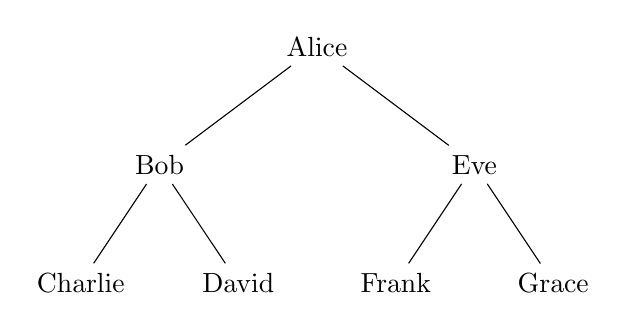
\begin{tikzpicture}[
      level 1/.style={sibling distance=40mm},  % Adjust the distance between siblings in level 1
      level 2/.style={sibling distance=20mm}   % Adjust the distance between siblings in level 2
    ]
        \node {Alice}
            child {node {Bob}
                child {node {Charlie}}
                child {node {David}}
            }
            child {node {Eve}
                child {node {Frank}}
                child {node {Grace}}
            };
    \end{tikzpicture}
    \caption{Family Tree}\label{fig:family-tree}
\end{figure}


This family tree has four generations: Alice, Bob, Charlie, David, Eve, Frank, and Grace. Alice is the parent of Bob and Eve, Bob is the parent of Charlie and David, and so on. The relationships between family members can be represented using a tree structure. Let's write an algorithm that accesses the children of a node in a family tree:

\begin{lstlisting}
# Accesses the children of a node in a family tree
# Args:
#     tree: The family tree to access
#     node: The node to access
# Returns:
#     The children of the node in the family tree

def access_children(tree, node):
    for parent, children in tree.items():
        if parent == node:
            return children

tree = {"Alice": ["Bob", "Eve"],
        "Bob": ["Charlie", "David"],
        "Eve": ["Frank", "Grace"]}
print(access_children(tree, "Bob"))  # Output: ["Charlie", "David"]
\end{lstlisting}

\newpage % Start the code snippet on a new page to avoid splitting it across pages

\section{Conclusion on Computer Science Foundations}

In this chapter, we discussed some fundamental concepts in computer science, such as algorithms and data structures. Algorithms are step-by-step procedures for solving problems, and data structures are ways of organizing data so that it can be used efficiently. We looked at some basic algorithms, such as the Pythagorean theorem, factorial, and Fibonacci sequence. We also discussed some common data structures, such as arrays, linked lists, and trees. These concepts are essential for understanding computer science and its applications in mathematics.


\chapter{Statistics}\label{chap:statistics}

\section{Introduction}

Statistics is a branch of mathematics that deals with the collection, analysis, interpretation, and presentation of data. In \textbf{CS} statistics is used to analyze data, make predictions, and draw conclusions. In this chapter, we will discuss the basic concepts of statistics and how they are used in computer science.

\section{Tabular Data}

Tabular data is a common way to represent data in statistics. A table consists of rows and columns, where each row represents a data point and each column represents a variable. For example, consider the following table of student grades:

\begin{table}[H]
\centering
\caption{Student Grades Across Subjects}
\begin{tabular}{|c|c|c|c|c|}
\hline
\textbf{Student} & \textbf{Math} & \textbf{Science} & \textbf{English} & \textbf{History} \\
\hline
Alice    & 85  & 90  & 88  & 82 \\
Bob      & 75  & 80  & 78  & 72 \\
Charlie  & 90  & 85  & 88  & 92 \\
David    & 80  & 75  & 82  & 78 \\
\hline
\end{tabular}\label{tab:student-grades}
\end{table}

In this table, each row represents a student, and each column represents a subject. The numbers in the table represent the grades of the students in each subject. This table can be used to analyze the performance of the students in different subjects. What would the table look like in code?

\begin{lstlisting}[caption={Student Grades Across Subjects in Python}, label={lst:student-grades}]
student_grades = {
    'Alice': [85, 90, 88, 82],
    'Bob': [75, 80, 78, 72],
    'Charlie': [90, 85, 88, 92],
    'David': [80, 75, 82, 78]
}
\end{lstlisting}

In Listing~\ref{lst:student-grades}, we use a Python dictionary to represent the student grades. The keys of the dictionary are the student names, and the values are lists of grades in different subjects. This data structure is useful for storing tabular data in Python.

\subsection{Summary Statistics}

Summary statistics are used to summarize the data in a table. Some common summary statistics include:

\begin{itemize}
    \item Mean: The average value of a variable.
    \item Median: The middle value of a variable.
    \item Mode: The most frequent value of a variable.
    \item Range: The difference between the maximum and minimum values of a variable.
    \item Variance: The average squared difference between each value and the mean.
    \item Standard Deviation: The square root of the variance.
    \item Correlation: The relationship between two variables.
    \item Covariance: The measure of how two variables change together.
    \item Percentile: The value below which a given percentage of observations fall.
    \item Quartile: The values that divide the data into four equal parts.
    \item Interquartile Range: The range between the first and third quartiles.
    \item Outlier: An observation that is significantly different from other observations.
    \item Skewness: The measure of the asymmetry of the data distribution.
    \item Kurtosis: The measure of the peakedness of the data distribution.
    \item Confidence Interval: The range of values that is likely to contain the true value of a parameter.
    \item \ldots and many more.
\end{itemize}

These summary statistics can be calculated using Python libraries such as NumPy, SciPy, and Pandas. Let's calculate the mean, median, and standard deviation of the student grades in Listing~\ref{lst:student-grades}.

lets calculate the mean, median, and standard deviation of the student grades in Listing~\ref{lst:student-grades}. First in math, then in code.

\subsection{Mathematical Calculation}
\[
\text{Math grades: } [85, 75, 90, 80]
\]
\begin{align*}
\text{Mean} &= \frac{85 + 75 + 90 + 80}{4} = 82.5 \\
\text{Median} &= \frac{80 + 85}{2} = 82.5 \\
\text{Standard Deviation} &= \sqrt{\frac{(85 - 82.5)^2 + (75 - 82.5)^2 + (90 - 82.5)^2 + (80 - 82.5)^2}{4}} = 5.59
\end{align*}

Now, let's calculate the mean, median, and standard deviation of the student grades using Python. Below is the code snippet to calculate the summary statistics.

\begin{lstlisting}[caption={Calculating Summary Statistics in Python}, label={lst:summary-statistics}]
student_grades = {
    'Alice': [85, 90, 88, 82],
    'Bob': [75, 80, 78, 72],
    'Charlie': [90, 85, 88, 92],
    'David': [80, 75, 82, 78]
}

def get_student_average(arr):
    return sum(arr) / len(arr)

def get_student_median(arr):
    arr.sort()
    n = len(arr)
    if n % 2 == 0:
        return (arr[n // 2 - 1] + arr[n // 2]) / 2
    else:
        return arr[n // 2]
    
def get_student_standard_deviation(arr):
    mean = get_student_average(arr)
    return (sum([(x - mean) ** 2 for x in arr]) / len(arr)) ** 0.5

def get_student_stats(student_grades):
    stats = {}
    for student, grades in student_grades.items():
        stats[student] = {
            'average': get_student_average(grades),
            'median': get_student_median(grades),
            'standard_deviation': get_student_standard_deviation(grades)
        }
    return stats

def print_student_stats(stats):
    for student, data in stats.items():
        print(f'{student}:')
        print(f'  Average: {data["average"]:.2f}')
        print(f'  Median: {data["median"]:.2f}')
        print(f'  Standard Deviation: {data["standard_deviation"]:.2f}')

print_student_stats(get_student_stats(student_grades))
\end{lstlisting}

In Listing~\ref{lst:summary-statistics}, we define three functions to calculate the average, median, and standard deviation of a list of numbers. We then define a function \texttt{get\_student\_stats} that calculates these statistics for each student in the \texttt{student\_grades} dictionary. Finally, we print the statistics for each student using the \texttt{print\_student\_stats} function.

\section{Sequential Equations}

Sequential equations are a set of equations that are solved in a sequence. In many cases, the solution to one equation is used as an input to another equation. You will notice that in math, sequential equations are very verbose and can be hard to follow. In computer science, we can represent sequential equations in a more concise and readable way using code. Let's consider an example of sequential equations in math and how they can be represented in Python. Don't pay much attention to the math, focus on the difference in representation.

\subsection{Example of sequential equations in math (verbose):}

\[
\begin{aligned}
    & \text{Given the initial value:} \\
    & x_1 = 5 \\
    & \text{Now, use } x_1 \text{ to calculate } x_2: \\
    & x_2 = 2x_1 + 3 = 2(5) + 3 = 13 \\
    & \text{Next, use } x_2 \text{ to calculate } x_3: \\
    & x_3 = x_2^2 - 4 = 13^2 - 4 = 169 - 4 = 165 \\
    & \text{Finally, use } x_3 \text{ to calculate } x_4: \\
    & x_4 = \sqrt{x_3 + 7} = \sqrt{165 + 7} = \sqrt{172} \approx 13.11
\end{aligned}
\]

This example shows how each equation depends on the result of the previous one. While these steps are explicit, they can become tedious, especially when there are many intermediate steps involved.

\subsection{Example of sequential equations in Python (concise):}


\begin{lstlisting}[caption={Sequential Equations in Python}, label={lst:sequential-equations}]
import math

# Initial value
x1 = 5

# Sequential equations
x2 = 2 * x1 + 3
x3 = x2**2 - 4
x4 = math.sqrt(x3 + 7)

print(f"x1: {x1}, x2: {x2}, x3: {x3}, x4: {x4}")
\end{lstlisting}

In Python, the process is much more concise and easier to follow. The verbosity of the mathematical solution is abstracted into code, allowing the focus to remain on the logic rather than the intermediate steps. Additionally, the ability to reuse code for similar problems makes this approach highly efficient.

This comparison illustrates how sequential equations, which can appear verbose and complex in mathematics, are simplified in programming due to abstraction and reuse of operations.

\section{Probability}

Probability is a measure of the likelihood that an event will occur. In computer science, probability is used to model uncertainty, make predictions, and analyze data. Let's discuss some basic concepts of probability and how they are used in computer science.

\subsection{Basic Probability Concepts}

Some basic probability concepts include:

\begin{itemize}
    \item Sample Space: The set of all possible outcomes of an experiment.
    \item Event: A subset of the sample space.
    \item Probability: The likelihood that an event will occur, denoted by $P(A)$.
    \item Complement: The probability that an event will not occur, denoted by $P(A')$.
    \item Union: The probability that either of two events will occur, denoted by $P(A \cup B)$.
    \item Intersection: The probability that both of two events will occur, denoted by $P(A \cap B)$.
    \item Conditional Probability: The probability of an event given that another event has occurred, denoted by $P(A|B)$.
    \item Independence: Two events are independent if the occurrence of one does not affect the occurrence of the other.
    \item Bayes' Theorem: A formula that describes the probability of an event based on prior knowledge.
\end{itemize}

These concepts are fundamental to understanding probability theory and are used in various applications in computer science, such as machine learning, data analysis, and cryptography.

\subsection{Probability Distributions}

Probability distributions describe how the probabilities of different outcomes are distributed. Some common probability distributions include:

\begin{itemize}
    \item Uniform Distribution: All outcomes are equally likely.
    \item Bernoulli Distribution: A distribution with two possible outcomes (e.g., success or failure).
    \item Binomial Distribution: A distribution of the number of successes in a fixed number of trials.
    \item Normal Distribution: A bell-shaped distribution with a mean and standard deviation.
    \item Poisson Distribution: A distribution of the number of events occurring in a fixed interval of time or space.
    \item Exponential Distribution: A distribution of the time between events in a Poisson process.
    \item \ldots and many more.
\end{itemize}

These distributions are used to model random variables and make predictions about the likelihood of different outcomes. In computer science, probability distributions are used in various algorithms, simulations, and statistical analyses.

\subsection{Example of Probability Calculation}

Let's consider an example of calculating the probability of rolling a six on a fair six-sided die. In this case, the sample space is $\{1, 2, 3, 4, 5, 6\}$, and the event of interest is rolling a six. The probability of rolling a six is given by:

\[
P(\text{Rolling a Six}) = \frac{\text{Number of favorable outcomes}}{\text{Total number of outcomes}} = \frac{1}{6}
\]

This example illustrates how probability can be calculated using the concept of favorable outcomes and the total number of outcomes. In computer science, this calculation can be implemented using code to simulate random events and calculate probabilities.

\subsection{Probability Calculation in Python}

Let's calculate the probability of rolling a six on a fair six-sided die using Python. We will simulate rolling the die multiple times and calculate the empirical probability based on the outcomes.

\begin{lstlisting}[caption={Probability Calculation in Python}, label={lst:probability-calculation}]
import random

def roll_die():
    return random.randint(1, 6)

def calculate_probability(n):
    favorable_outcomes = 0
    total_outcomes = 0
    for _ in range(n):
        outcome = roll_die()
        if outcome == 6:
            favorable_outcomes += 1
        total_outcomes += 1
    return favorable_outcomes / total_outcomes

n = 10000
probability = calculate_probability(n)
print(f"Empirical Probability of Rolling a Six: {probability:.4f}")
\end{lstlisting}

In Listing~\ref{lst:probability-calculation}, we define a function \texttt{roll\_die} to simulate rolling a fair six-sided die and a function \texttt{calculate\_probability} to calculate the empirical probability of rolling a six based on a given number of trials \texttt{n}. We then print the empirical probability of rolling a six based on 10,000 trials.

This example demonstrates how probability calculations can be implemented in Python using random simulations and empirical data.

\section{Conclusion of Statistics}

Statistics is a powerful tool for analyzing data, making predictions, and drawing conclusions. In computer science, statistics is used to model uncertainty, optimize algorithms, and analyze complex systems. By understanding the basic concepts of statistics and how they are applied in computer science, you can gain valuable insights into the world of data science, machine learning, and artificial intelligence. In the next chapter, we will explore the field of linear algebra and its applications in computer science.



\end{document}
